\documentclass[landscape]{article}
\usepackage[a4paper,landscape,margin=1.5cm]{geometry}
\usepackage{graphicx}
\usepackage{array}
\usepackage{tabularx}
\usepackage{colortbl}
\usepackage{xcolor}
\usepackage{fancyhdr}
\usepackage{tikz}
\usepackage{booktabs}
\usepackage{subcaption}
\usepackage{pagecolor}

\graphicspath{{illustration/}{reference/}}  % DO NOT CHANGE THIS LINE

% Define custom colors
\definecolor{headerred}{RGB}{255,0,0}
\definecolor{lightgreen}{RGB}{240,255,240}
\pagecolor{lightgreen} % Set background color

% Custom page style
\pagestyle{fancy}
\fancyhf{}
\renewcommand{\headrulewidth}{0pt}
\cfoot{\textcolor{headerred}{\thepage}} % Added page number in footer center

\begin{document}
% Header Section
\begin{center}
\Huge\bfseries\sffamily\textcolor{headerred}{TECHNICAL SPECIFICATION SHEET}
\end{center}

\vspace{0.5cm}

% PRODUCT DETAILS
\noindent\begin{tabularx}{\textwidth}{|X|X|X|X|}
\hline
\rowcolor{headerred}\multicolumn{4}{|c|}{\textcolor{white}{\textbf{PRODUCT DETAILS}}} \\
\hline
Brand Name: W & Designer: William & Season: Spring/Summer & Category: Outerwear \\
\hline
Date: 2025-03-09 & Style Name: Modern Jacket & Style Number: MJ2025 & Main Fabric: Cotton \\
\hline
\end{tabularx}

\vspace{0.5cm}

% STYLE DESCRIPTION
\noindent\begin{tabularx}{\textwidth}{|X|}
\hline
\rowcolor{headerred}\multicolumn{1}{|c|}{\textcolor{white}{\textbf{STYLE DESCRIPTION}}} \\
\hline
A contemporary jacket with a sleek design, featuring a minimalist silhouette and lightweight cotton fabric ideal for spring and summer seasons.
\end{tabularx}
\hline

\vspace{0.5cm}

% TECHNICAL DRAWINGS
\noindent\begin{tabularx}{\textwidth}{|X|}
\hline
\rowcolor{headerred}\multicolumn{1}{|c|}{\textcolor{white}{\textbf{TECHNICAL DRAWINGS}}} \\
\hline
\begin{center}
% First row of drawings
\begin{tabular}{cc}
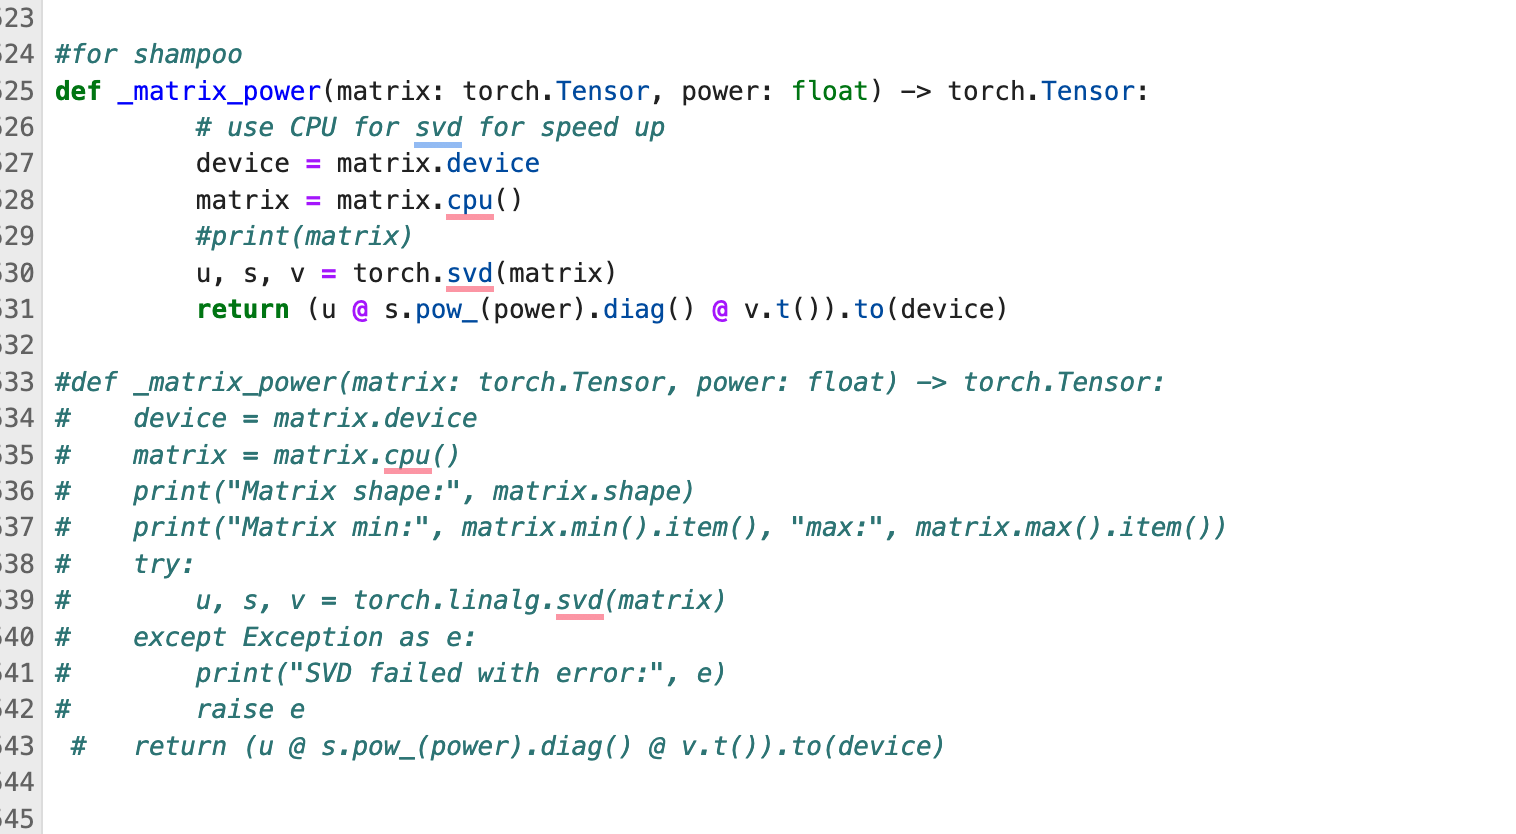
\includegraphics[width=0.4\textwidth,height=8cm,keepaspectratio]{Screenshot_2025-03-09_at_15.26.02.png} &
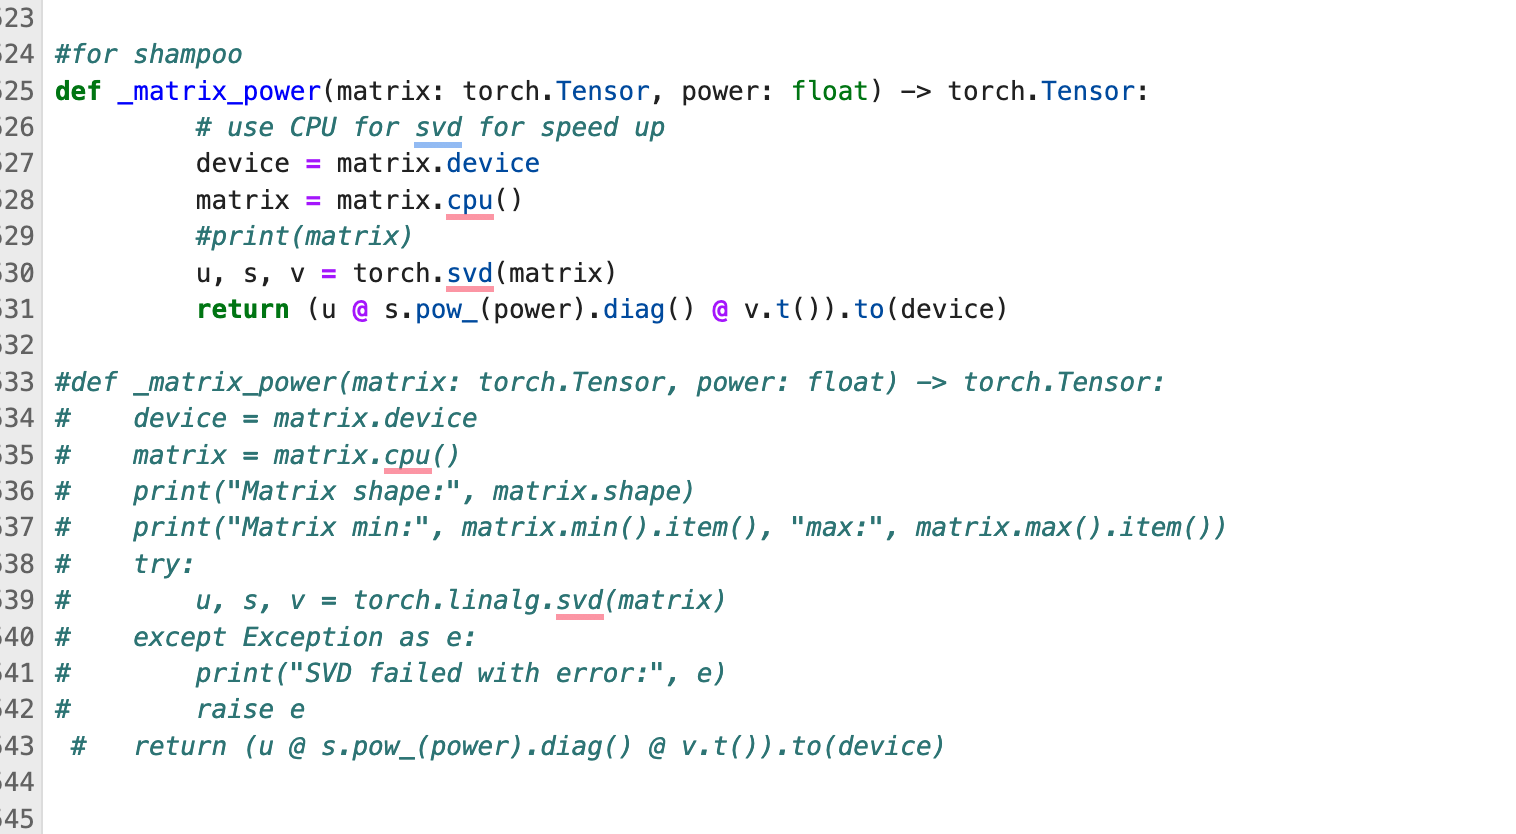
\includegraphics[width=0.4\textwidth,height=8cm,keepaspectratio]{Screenshot_2025-03-09_at_15.26.02.png} \\
\end{tabular}
\end{center}
\end{tabularx}
\hline

\vspace{0.5cm}

\newpage
% MEASUREMENTS
\noindent\begin{tabularx}{\textwidth}{|X|X|X|X|X|X|X|}
\hline
\rowcolor{headerred}\multicolumn{7}{|c|}{\textcolor{white}{\textbf{MEASUREMENTS}}} \\
\hline
\textbf{Item} & \textbf{Description} & \textbf{XS} & \textbf{S} & \textbf{M} & \textbf{L} & \textbf{XL}\\
\hline
Sleeve Length & Full-length sleeve, cotton & 60 cm & 62 cm & 64 cm & 66 cm & 68 cm \\
\hline
Chest Width & Across chest, cotton & 48 cm & 50 cm & 52 cm & 54 cm & 56 cm \\
\hline
Jacket Length & From shoulder to hem, cotton & 65 cm & 67 cm & 69 cm & 71 cm & 73 cm \\
\hline
\end{tabularx}

\vspace{0.5cm}

% CARE INSTRUCTIONS
\noindent\begin{tabularx}{\textwidth}{|X|}
\hline
\rowcolor{headerred}\multicolumn{1}{|c|}{\textcolor{white}{\textbf{CARE INSTRUCTIONS}}} \\
\hline
\begin{itemize}
    \item Machine wash cold with like colors.
    \item Use non-chlorine bleach when needed.
    \item Tumble dry low.
    \item Iron on low heat if necessary.
    \item Do not dry clean.
\end{itemize}
\end{tabularx}
\hline

\vspace{0.5cm}

% ADDITIONAL COMMENTS
\noindent\begin{tabularx}{\textwidth}{|X|}
\hline
\rowcolor{headerred}\multicolumn{1}{|c|}{\textcolor{white}{\textbf{ADDITIONAL COMMENTS}}} \\
\hline
This works
\end{tabularx}
\hline

\end{document}